\chapter{Introduction}

\section{Real-Time Systems}

Computer systems consist of a combination of hardware, software, user and data. Such
systems are constantly evolving and will become undoubtedly a constituent part of our daily 
lives.
Nowadays, computer systems are widespread in several application domains. From simple systems
like espresso machines to complex larger systems such as an airplane, these systems are
continuously developing to facilitate and enhance our lifestyle by always providing improved 
solutions (more comfort, energy efficient, security, etc.) that answer directly to real life 
problems.  
\emph{Real-time} systems are defined as those systems in which the correctness of the system
depends not only on the logical results of computations, but also on the physical time at which 
the results are produced~\cite{intro:stan88}.
In other terms, real-time systems are computing systems that have temporal constraints to meet
and thus, are required to guarantee a response within specified timing constraints. 
Such systems need to achieve different requirements that can be structured into three main 
categories~\cite{intro:kopetz11}: \emph{(i)} functional requirements, 
\emph{(ii)} temporal requirements, and \emph{(iii)} dependability requirements.
Functional requirements refer to the functions that the real-time system must perform. 
In order to accomplish such requirements, the system needs to be able to observe its current
state, that is, the values of variables describing the latter. For instance the position, speed
and level of oil in a car are possible state variables. Additionally, a given system 
needs to control its state variables (actuation) for regulation purposes, and provide an 
interface to the system operator that allows its monitoring.
On the other hand, temporal requirements are born from the requirements of control loops. 
A typical example is the time bounds for which a gear change needs to be achieved in the control
system operating in modern vehicles. Temporal requirements of a given system might be of
different order of magnitude. For instance the man-machine interface, in comparison with fast
control loops, is less strict because of the human perception of time. Finally, dependability
requirements are additional requirements regarding the quality of service that a given system
produces, that is, the criteria for deciding whether the services provided by the system can 
justifiably be trusted. The concept of dependability encompasses the following attributes
\cite{intro:aviz04}: availability (readiness for correct services), reliability (continuity of
correct services), safety (absence of catastrophic consequences), integrity (absence of 
improper system alterations), and maintainability (ability to undergo modifications and repairs).

Real-time systems can be classified from different perspectives~\cite{intro:kopetz11} based
on either the characteristics of the application (perspective A), i.e., on factors outside 
the computer system, or on the design and implementation (perspective B), i.e., on factors 
inside the computer system.
Tables~\ref{tab:rts_class} presents a classification of real-time systems based on these two 
perspectives:
\begin{table}[!h]
  \begin{tabular}{ |c|c|c| } 
    \hline
    Perspective  & Classification & Description \\
    \hline
    \multirow{2}{*}{A} & \makecell{hard real-time \\ vs \\ soft real-time} 
                         & \parbox{0.55\linewidth}{\vspace{1mm}A hard real-time system is a \
                         system that must meet
                         \emph{hard deadlines}, that is, deadlines that if missed could result
                         in severe consequences. On the other hand, for 
                         soft real-time systems the goal becomes to meet a certain subset
                         of deadlines in order to optimize some specific criteria. Particularly,
                         deadline violations result in degraded quality. However, the system 
                         keeps operating and may recover in the future.
                         \vspace{1mm}} \\ \cline{2-3} 
                         & \makecell{fail-safe \\ vs \\ fail-operational}
                         & \parbox{0.55\linewidth}{\vspace{1mm}Fail-safe systems refer to those 
                         systems where a safe state can be identified and quickly reached 
                         upon the occurrence of a failure. On the contrary, fail-operational 
                         systems
                         are systems that must remain operational and provide a minimal level
                         of service even in case of failure (no safe state).\vspace{1mm}} 
                        \\ \cline{2-3} 
    \hline\cline{1-3}\hline
    \multirow{3}{*}{B} & \makecell{guaranteed-response \\vs\\ best effort}
                         & \parbox{0.55\linewidth}{\vspace{1mm}Real-time systems where the 
                         probability of failure is reduced to the probability that some
                         assumptions, on peak load or fault number and types for instance, 
                         do not hold in reality are called guaranteed-response. On the other 
                         hand, best-effort systems are systems where no analytical arguments for 
                         correctness can be made. The latter is rather established during the
                         test and integration phases.\vspace{1mm}} \\ \cline{2-3} 
                         & \makecell{resource-adequate\\ vs\\ resource-inadequate}
                         & \parbox{0.55\linewidth}{\vspace{1mm}While Resource-adequate systems
                         are systems that provide sufficient computational resources to handle
                         a specified peak load and fault scenarios, resource-inadequate 
                         systems rely on dynamic resource allocation strategy. It is based on 
                         resource sharing and probabilistic arguments about expected load and 
                         fault scenarios.\vspace{1mm}} \\ \cline{2-3} 
                         & \makecell{event-triggered\\ vs\\ time-triggered}
                         & \parbox{0.55\linewidth}{\vspace{1mm}Event-triggered systems are 
                         systems where all communication and processing activities are initiated
                         whenever a significant event (rather than the regular clock tick) 
                         occurs. Oppositely, in time-triggered systems all activities are 
                         initiated by the progress of real-time.\vspace{1mm}} \\ \cline{2-3} 
    \hline
  \end{tabular}
  \caption{Classification Of Real-Time Systems}
  \label{tab:rts_class}
\end{table}

\section{Control Aspects in Real-Time Systems}

\subsection{Temporal Control Versus Logical Control}
When building real-time systems, a clear distinction between the aspects related to the time 
domain and those related to the value domain needs to be made. The latter are respectively
referred to as the concepts of \emph{temporal control} and \emph{logical control}.
Temporal control is related to the progression of \emph{real-time}. It is of concern when it 
comes to determining the instants in the domain of real time for the accomplishment of 
computations, that is, when computations must be activated.
Such instants are derived from the dynamic of the application. 

Logical control is related to the control flow \emph{within} a given task, meaning that it 
is based on the given task structure and the particular input data. For instance, the execution
of a branch condition and the selection of one of the alternatives is an example of logical
control. The \emph{execution time} represents the time interval needed to execute a task
performing the logical control.
If the temporal control and the logical control aspects are mixed in a program segment,
then it is impossible to determine the worst-case execution time of this program segment without
analyzing the behavior of its environment.
\begin{example}\label{exp:control1}
 A semaphore wait statement is a temporal control statement. If a semaphore
wait statement is contained in a program segment that also includes logical control
(algorithmic) statements, then the temporal behavior of this program segment depends
on both, the progress of execution time and the progress of real-time.
\end{example}
Thus, a good design decouples the reasoning about temporal constraints, governed by the 
application, from the reasoning about logical inner aspects of the algorithmic part of the 
application.
Synchronous real-time languages, such as LUSTRE~\cite{intro:lustre} and 
ESTEREL~\cite{intro:esterel} distinguish clearly between logical control and temporal
control. In these languages, the progression of real-time is partitioned into an
(infinite) sequence of intervals of specified real-time duration, which we call
steps. Each step begins with a tick of a real-time clock that starts a computational
task (logical control). The computational model assumes that a task, once activated
by the tick of a real-time clock (temporal control), finishes its computation quasi
immediately. Practically, this means that a task must terminate its execution before
the next triggering signal (the next tick of the real-time clock) initiating the next
execution of the task.

\subsection{Event-Triggered Control Versus Timed-Triggered Control}
In real-time systems, the activation (start-up) of computation tasks is usually achieved through
triggering signals, that is, control signals that specify the instant when an activity 
(computation) should start in the temporal domain.
Two main paradigms are commonly used for triggering activities of a real-time system, namely,
the event-triggered control and the time-triggered control.
We say that the control is event-triggered when the triggering signal is associated to 
the occurrence of a significant event, such as the arrival of a particular message, the 
fulfillment of an activity within a component, or the occurrence of an external interrupt.
Time-triggered control relies on the progression of time. The activation of computation is 
pre-determined and usually depends on the periodic overflow of a timer.
Time-triggered systems are based on the notion of \emph{logical execution time (LET)} 
introduced by the programming language Giotto~\cite{intro:giotto}. LET specifies the amount of 
time between the activation time of a computation and its due time. It abstracts the execution
time of programs in the sense that even if they start before their activation date 
and finish before their due time, they behave as if they exactly consumed their LET.

\section{System Design}
System design is the process of defining the elements of a system such as the requirements, 
the architecture, the system components and their interfaces as well as the data flowing 
through the system.
System design implies a systematic approach to the design of a system. It may adopt a bottom-up 
or a top-down approach, but either way the process is systematic wherein it takes into account 
all
related variables of the system that need to be created. From the architecture, to the required 
hardware and software, right down to the data and how it travel and transform throughout its 
travel through the system. System design, then, overlaps with system analysis, system 
engineering and system architecture.
The system design approach first appeared right before World War II, when engineers were 
trying to solve complex control and communication problems. They needed to be able to 
standardize their work into a formal discipline with proper methods, especially for new fields 
like information theory, operational research and computer science in general.

System design~\cite{intro:sys_design} differs radically from pure software design in the sense
that it does not focus only on functional requirements. It also accounts for nonfunctional 
properties such as timing, energy consumption, or even fault tolerance. Meeting such 
extra functionalities is essential and requires evaluation of how design choices affect 
the overall system behavior. 

\subsection{Design Flows}
Design of real-time systems is a rather complex task~\cite{intro:sys_design2} which has to be 
broken down into a number of subtasks. In theory, the design process should be structured into
distinct phases starting from the analysis phase until the final validation of the system and 
its effective deployment. In practice, such a strict sequential decomposition 
is hardly possible.
In fact the design flow is rather decomposed into several iterations as depicted in 
Figure~\ref{fig:design}. Each iteration needs to include test generation and an evaluation 
of testability. A given design is then evaluated with respect to the different objectives 
(performance, dependability, energy consumption, etc.). 
\begin{figure}[h!]
\centering
\begin{tikzpicture}




   \fill[even odd rule,gray!35] circle (2.5);

   \node at (0,0) [
      font  = \mytextstyle,
      color = white,
      align = center
   ](mid){\Large\textbf  Design Flow};
   
  \arcarrow{130}{100}{Analysis}{cyan!30}
   \arcarrow{97}{67}{Feedback}{red!20}
   \arcarrow{64}{40}{Design}{green!30}
   \arcarrow{37}{7}{Feedback}{red!20}
   \arcarrow{4}{-44}{Implementation}{blue!30}
   \arcarrow{-47}{-77}{Feedback}{red!20}
   \arcarrow{-80}{-116}{Integration}{orange!30}
   \arcarrow{-119}{-149}{Feedback}{red!20}
   \arcarrow{-152}{-190}{Deployment}{yellow!30}
   \arcarrow{-193}{-225}{Feedback}{red!20}

  \node[above=4 of mid,xshift=-4.5cm](spec) {Specifications};
  \node[below=4 of mid,xshift=4.5cm,align=center](dep) {Acceptance Testing \\ 
  and Final Deployement };


\node[single arrow, rounded corners=1pt,blue, fill=blue!30, draw, align=center,
  minimum height=12.5mm,minimum width=2mm,rotate=-45,below=4mm of spec,yshift=10mm,
  xshift=10mm](aw1){};

  
\node[single arrow, rounded corners=1pt,blue, fill=blue!30, draw, align=center,
  minimum height=12.5mm,minimum width=2mm,rotate=-45,above=4mm of dep,yshift=-10mm,
  xshift=-10mm](aw1){};




\end{tikzpicture} 
\caption{Overal Design Flow}
\label{fig:design}
\end{figure}



\subsection{Design Styles}

In what follows, we present some important design styles used in the design of real-time systems.
Notice that the presented design styles are not exclusive in the sense that a given approach
may combine several design styles.

\subsubsection{Model-Based Design}
Model-based design~\cite{intro:mb,intro:mb2} is one promising approach in building 
real-time systems. It relies on mathematical modeling for the design, analysis 
and validation of systems. This approach captures not only what the dynamic and the 
expected properties of the system are, but also what is assumed about the system's environment.
Thus, It enables developers to verify the logic of their
application, assumptions about its environment and end-to-end behavior at early stages of the
design cycles.
First, an application model expressing the behavior and dynamic of the considered system is 
built. It represents an abstraction that is platform independent, meaning that it does not 
consider any hardware specification such as communication delays or CPU(s) speed, which allows 
to model the system at early stages without any knowledge of the target platform, 
verify the obtained model against some safety properties (functional requirements), or even
to synthesize a control strategy for tuning the system.
Thereafter, the application source code, which represents the actual 
implementation of the system on a given platform, is automatically generated from the high 
level model, and integrated in a simulated environment. 

\subsubsection{Component-Based Design}

Large scale systems are complex systems that usually require to assemble several
components with wide-range functionalities. Many issues may rise when designing such 
systems~\cite{intro:cb} ranging from the design process and the relationships with suppliers to 
incomplete specifications and testing. A typical example is the Toyota sticky accelerator 
problem that was caused in part by components provided by two contractors whose interaction 
was not verified appropriately.
Component-based design tackles these issues by proposing an approach where such systems
are build by assembling strongly encapsulated entities called \emph{component} with 
stable, well-defined, and rigorous interface specifications~\cite{intro:cb2}.
This approach is based on the principle of re-usability of heterogeneous components and focuses
on the idea that internal knowledge about the design or the implementation of the latter is
not needed. In some cases, this knowledge is not even available. 

\subsubsection{Architecture-Based Design}

A system architecture is a conceptual model that describes the structure, behavior, and 
constraints 
of a system along with the interaction with its environment. Designing the architecture of 
a system is acknowledged to be a very hard task since it must address practical concerns
of the engineering efforts~\cite{intro:ab2} involved in system development (short term) 
and evolution (long term). Moreover, it needs to support a set of requirements whose
details may be unknown until an advanced late step of the development process. 
Thus, a methodical design approach that provides means for coping with requirements uncertainty,
and proposes guidance that helps in the decision making during the design process, is needed.
Architecture-based design~\cite{intro:ab} helps not only to detect design errors early in the 
development process, but also supports engineering efforts, which allows to produce 
high-quality code, by addressing the aforementioned problems.

\section{Existing Approaches For Building Real-Time Systems}

\subsection{Giotto}
Giotto~\cite{intro:giotto} is a programming approach for representing embedded systems
at the architecture level using a timed-triggered programming language. It separates the
platform-independent functionalities and timing aspects from platform-dependent scheduling 
and communication issues. It allows thus, an intermediate abstraction that enables the 
design engineers to annotate the functional programming modules with temporal attributes that 
are derived from the high-level stability analysis of control loops. 
Figure~\ref{fig:giotto} depicts the workflow of Giotto. A platform-abstract Giotto program
is written. This program captures all the functionalities and the timing aspects necessary
for ensuring consistency with the mathematical model of the control design. Thereafter,
the program is implemented on a given platform. Notice that this step is completely decoupled
from the first step in the sense that it does not require any interaction with the control 
engineer, and can in large parts be automated using powerful compilers. 
Giotto compilation facilitates the evaluation and the optimization phases by guarantying 
the preservation of functionalities and timings. 
\begin{figure}[h!]
\centering
\begin{tikzpicture}

\node(a){Control Design};
\node[below=7.5mm of a,rotate=-90](aa){$\Rightarrow$};
\node[below=7.5mm of aa,xshift=4mm](b){Giotto Program};
\node[below=7.5mm of b,rotate=-90](bb){$\Rightarrow$};
\node[below=7.5mm of bb,align=center,xshift=4mm](c){Code for Real-Time\\ Platform};
\node[right=3cm of a,align=center]{\vbox{\begin{itemize}
\item Modeling
\item Control law derivation
\end{itemize}}};

\node[right=29.5mm of b,align=center]{\vbox{\begin{itemize}
\item Functionalities and timings 
\item Periodic software tasks and mode switches
\end{itemize}}};

\node[right=27mm of c,align=center]{\vbox{\begin{itemize}
\item Hardware mapping
\item Computation and communication scheduling
\end{itemize}}};


\end{tikzpicture} 
\caption{Giotto Workflow}
\label{fig:giotto}
\end{figure}

In Giotto, all data are communicated through ports that can be classified into three categories:
sensor ports, actuator ports and task ports. Sensor ports are updated by the environment, 
whereas all other ports are updated by the Giotto program. Task ports are used to communicate 
data between concurrent tasks or to transfer data from one mode (execution mode) to another.
A Giotto task consists of a set of \texttt{In} (input) ports, a set of \texttt{out} (output)
ports, and a function \texttt{f} from its input ports and current state, which can be viewed
as a set of private ports inaccessible from outside the task, to its output ports
and its next state. 
The invocation of Giotto tasks are based on two essential concepts: instantaneous communication
and time determinism. In fact, tasks are activated on periodic cycles P 
(Figure~\ref{fig:giottote}). The Giotto logical abstraction 
does not specify when and how the actual computation of a task \texttt{f} is performed, 
it only determines the instant at which input are read $t_{start}$ and output are produced 
$t_{end}$.
\begin{figure}[h!]
\centering
\begin{tikzpicture}



\draw[->]  (-2,0) -- (8,0) node[below left] {time};
\draw[-]   (-2,0) -- (-2,5) node[above left] {Tasks};
  \draw[-]  (2,0) -- (2,0.2) node[below,yshift=-2mm]{P};

\draw[-]  (-2,1) -- (8,1) ;
\draw[-]  (-2,2.5) -- (8,2.5) ;


  \draw[pattern=north east lines,pattern color=red!40,draw=red] (-2,2.5) rectangle (-1.5,1);
  \draw[pattern=north east lines] (-1.25,2.5) rectangle (1,1);
  \draw[pattern=north east lines,pattern color=green!40,draw=green] (1.5,2.5) rectangle (2,1);
  
  \node at (-.5,4)(i){Read Inputs};
  \node at (3,4)(o){Write Outputs};
  \node at (0,-1)(e){Task Execution};

  \draw[->] (i) -- (-1.75,2.5);
  \draw[->] (o) -- (1.75,2.5);
  \draw[->] (e) -- (0,1);


\end{tikzpicture} 
\caption{Example of a Giotto Task Execution}
\label{fig:giottote}
\end{figure}


\subsection{Oasis}

Oasis~\cite{intro:oasis1,intro:oasis2} is a framework that provides methods for the design 
and implementation of safety-critical real-time systems. It includes a complete set of 
development tools (code generation, validation, simulation and execution) that eases the design 
and verification stages
while complying with general standards. The Oasis approach relies on the time-triggered concept
to build systems that are fully deterministic, predictable, and reproducible in both the logical
and temporal domains, even in case of failure.
An Oasis application consists of a static set of communicating agents, i.e., autonomous execution
entities including processing operations. The execution of a processing operation is 
time-triggered on a time window that is automatically deduced form the agent's timing.
Every Oasis agent has an associated real-time window during which input and output data are 
visible.

Figure~\ref{fig:oasis} illustrates the execution of a processing operation within its time
interval: each processing operation performed by an
agent takes place between two temporal instants (points) of the real-time. 
These points are the beginning date ($t_{start}$), which is the earliest instant
when the processing can be started, and the ending date ($t_{end}$) which is the latest
date when it must be terminated. These two dates allow to explain a formal duration 
that is constant and represents a constraint for the actual duration of execution.
\begin{figure}[h!]
\centering
\begin{tikzpicture}



\draw[->]  (0,0) -- (10,0) node[below left] {real-time};
\draw[-]  (3.5,0.2) -- (3.5,-0.2)node[below]{$t_{start}$} ;
\draw[-]  (7,0.2) -- (7,-0.2)node[below]{$t_{end}$} ;
\draw[pattern=north east lines] (4,-0.2) rectangle (6,0.2) node[below,yshift=-5mm,xshift=-8mm]{$Processing_1$};


\end{tikzpicture} 
\caption{Execution of a Processing Operation in Oasis}
\label{fig:oasis}
\end{figure}




\subsection{PTIDES}
PTIDES~\cite{intro:ptides2} is an event-triggered 
programming model that serves as a coordination language for 
model-based design of distributed real-time embedded systems. 
It leverages network time synchronization to provide a coherent global temporal semantics.
PTIDES builds on top of a strong timed semantic foundation, based on discrete-event (DE)
model~\cite{intro:ptides4}, and provides a mathematical framework
for presenting strategies that explore concurrency of implementations. It also allows 
deterministic schedulability analysis.
PTIDES structures real-time software as an interconnection of components communicating using
timestamped events. 

Figure~\ref{fig:ptides} (taken from~\cite{intro:ptides}) illustrates the PTIDES workflow.
\begin{figure}[h]
  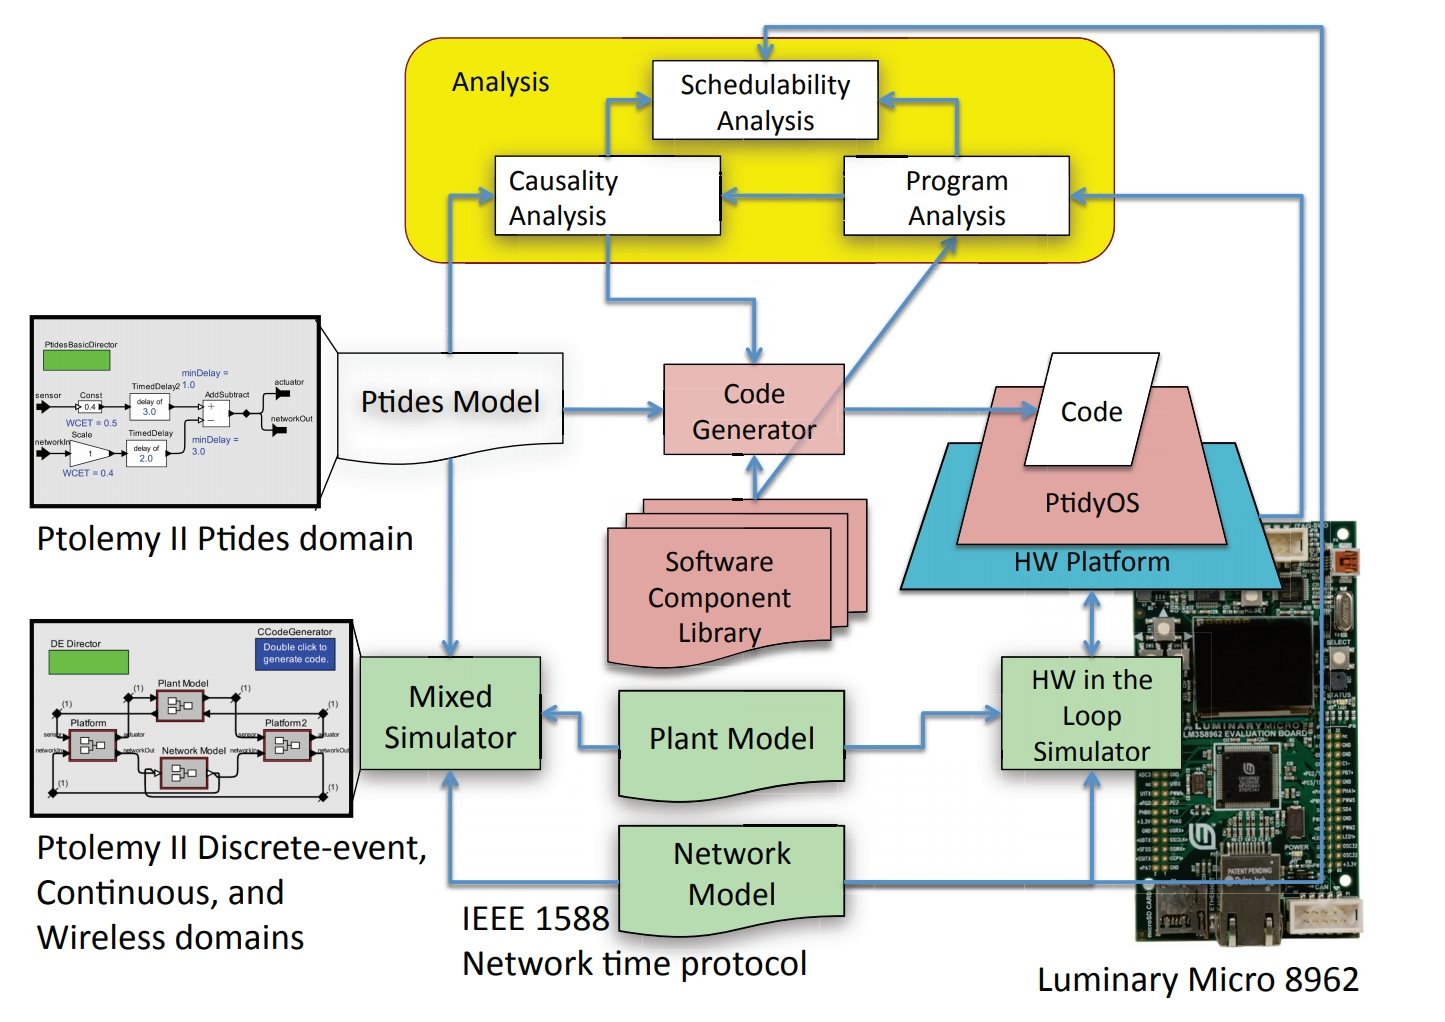
\includegraphics[scale=0.3]{Figures/ptides}
  \caption{PTIDES Code Generation and Analysis Workflow}
  \label{fig:ptides}
\end{figure}

The PTIDES design environment is an extension of the Ptolemy II framework~\cite{intro:ptides3},
which supports modeling, simulation, and design of systems using mixed models of computation. 
The physical part of the system can be modeled in the continuous domain. The simulation can be 
instantiated with different ODE solvers that suit diverse time scales present in the model. 
PTIDES models define the functional and temporal interaction of distributed software components,
the networks that bind them together, sensors, actuators, and physical dynamics. 
Simulation can be done on such models, such that functionality and timing can be 
tested. In particular, to get a picture of the temporal behavior
of a particular implementation of a model, each actor can
be endowed with a platform-dependent execution time, and
simulation can be performed to determine whether real-time
deadlines can be met for a given set of inputs.


\subsection{Lustre}
Lustre~\cite{intro:lustre} is a synchronous dataflow language used for the development of 
reactive systems, that is, systems that continuously interact with their environment.
The behavior of a Lustre program is a sequence of reactions consisting in reading the current 
inputs, computing the current outputs, and updating the internal state of the program. 
Lustre is based on the synchrony hypothesis~\cite{intro:lustre2}: A reaction is often said to 
\emph{take no time}. In other words, this means that a given system is faster than its 
environment. 

A Lustre program consists in a set of nodes operating on flows of values (inputs and outputs 
are described by their flows of values along with time). 
The synchronous dataflow approach consists in adding a time dimension to the dataflow model.
This is done by associating time with the rate of dataflow, that is, the manipulated entities
can be interpreted as function of time.
For instance, given a variable or an expression $x$,
it represents an infinite sequence of values $(x_0,\ldots,x_n,\ldots)$, $x_n$ being the value
of $x$ at the logical time instant n, that is, at the $n$-th  reaction of the program. 
Figure~\ref{fig:lustre3} shows a small example of a Lustre program.
\begin{figure}[H]
\begin{lstlisting}[basicstyle=\ttfamily,
escapeinside={||},
mathescape=true,
numbers=left,
backgroundcolor=\color{gray!20}]
  |\textbf{node}| Nand(X,Y: |\textbf{bool}|) |\textbf{returns}| (Z: |\textbf{bool}|);
     |\textbf{var}| U: |\textbf{bool}|;
  |\textbf{let}|
     U = X |\textbf{and}| Y;
     Z = |\textbf{not}| U;
  |\textbf{tel}|
\end{lstlisting}
\caption{A Lustre Program}
\label{fig:lustre3}
\end{figure}
The above program defines a node that takes two Boolean inputs X and Y, and returns the negation
of \say{X and Y}. It expresses the following relation:
\begin{displaymath}
  \text{For any instant t, \texttt{$Z_t$= not ($X_t$ and $Y_t$)}} 
\end{displaymath}

\section{Contribution}

Nowadays, real-time systems are ubiquitous in several application domains, 
and such an emergence led to an increasing need of performance: resources, 
availability, concurrency, etc. This expansion initiates a shift from the
use of single processor based hardware platforms, to large sets 
of interconnected and distributed computing nodes. Moreover, it prompts the birth 
of a new family of systems that are intrinsically distributed, namely, 
\emph{Networked Embedded Systems}. 
Such an evolution stems from an increase in complexity of real-time software 
embedded on such platforms (e.g. electronic control in avionics 
and automotive domains~\cite{charette09}), and the need to integrate 
formerly isolated systems~\cite{kopetz04} so that 
they can cooperate as well as share resources improving thus functionality 
and reducing costs.
To deal with such complexity, the community of safety critical systems 
often restricts its scope to predictable systems, which are represented 
with domain specific models (e.g. periodic tasks, synchronous systems, 
time-deterministic systems) for which the range of possible executions 
is small enough to be easily analyzed, allowing the pre-computation 
of optimal control strategies.
\emph{Networked Embedded Systems} usually describe a set of real-time systems, 
distributed across several platforms, and interacting through a network. 
Because of their adaptive behavior, the standard practice when implementing 
such systems is not to rely on models for pre-computation of execution strategies but rather 
to design systems dynamically adapting at runtime to the actual context of execution.
Such approaches, however, do not offer any formal guarantee of timeliness. Also, 
the lack of a priori knowledge on system behavior leaves also little room for 
static optimization.

In this thesis, we propose a rigorous design flow intended for building distributed real-time 
applications using the BIP Framework. BIP~\cite{intro:bip} (Behavior, Interaction, Priority)
is a model-based and component-based framework where systems consist of components
represented as timed automata that may synchronize on particular actions to coordinate
their activities.
Particularly, we investigate timed automata based models, with well defined semantics, in order 
to study the behavior of a given system with some imposed timing constraints when deployed 
in a distributed environment. 

\subsection*{Knowledge Based Optimization of}

In Chapter~\ref{chap:3}, we propose an intermediate model more appropriated for the 
representation of distributed real-time systems. It provides details on how the 
implementation of a system with multiparty interactions can be derived by explicitly expressing
the ongoing communication mechanism. This model is obtained using model transformations that
are in partly based of the notion of \emph{conflicting interactions}. In other words,
in a distributed context components may compete on the same resources at the same time. Thus,
any distributed implementation must preserve the overall system consistency by ensuring 
mutual exclusion in such cases. In fact, \emph{conflicts} are hard to characterize for real life
case studies and their computation is based on over-approximation. Chapter~\ref{chap:4} proposes
a knowledge based optimization in order to optimize the computation of the conflicting 
interactions set.


\subsection*{Communication Delays}

Chapter~\ref{chap:5} tackles the communication delays problem inherent to distributed real-time
systems. This is achieved by considering additional delays between the decision to execute 
an interaction and its actual execution. These delays result from the transmission
delays between the component responsible for such a decision and the components involved in
the interaction, and may have a huge impact in the satisfaction of timing constraints in 
real-time.
This will particularly help to anticipate the execution of interactions at 
least some delay beforehand, corresponding to the actual worst estimation of communication 
delays of a given platform, which will alleviate the effect of those delays on the system 
behavior.
Indeed, such delays may introduce behavioral flaws (e.g. deadlocks) when dealing with
arbitrary timing constraints (i.e. no restriction to the non-decreasing deadlines case
as in~\cite{ahlem_these}). The proposed approach introduces a semantics based on partial states
of the system components and formalizes in a precise way the effect of the delays
in this context. It also provides practical means for enforcing system correctness in their 
presence. 

\subsection*{Clock Drift}

The verification of real-time systems against some considered properties relies on the fact
that clocks are perfectly synchronous, that is, clocks advance at the same rate, which is not the
case in practice. Clocks are in fact implemented using oscillators and counter registers, thus,
their precision depend highly on the quality of the oscillators and parameters of their 
underlying environment (temperature, humidity, etc.). Chapter~\ref{chap:6} studies the 
effect of this hardware imperfections by breaking the perfect clocks assumption.
More precisely, this problem is formulated as a robustness problem, i.e., does the system
still satisfies the specification when subject to different kind of perturbations (in our case
clock imperfection). First, a timed automata model for distributed real-time system with 
drifting clocks is introduced. Thereafter, we revisit the robustness by proposing a strategy
that allows to have \say{similar} or close execution scenarios in the latter and the system with 
perfect clocks.

\section{Outline}
The rest of this thesis is structured as follows:
\begin{itemize}
  \item Part I introduces all the preliminaries and includes the following chapters:
    \begin{itemize}
      \item Chapter~\ref{chap:2} gives formal definitions of timed transition systems,
        timed automata, their semantics and properties.
      \item Chapter~\ref{chap:3} presents an intermediate timed automata based model for 
        the representation of distributed real-time systems. It also tackles two important
        constraints related the distributed real-time context.
    \end{itemize}
  \item Part II includes our contributions. It consists of the following chapters:
    \begin{itemize}
      \item Chapter~\ref{chap:4} proposes a knowledge based optimization for systems modeled
        using the approach of Chapter~\ref{chap:3}.
      \item Chapter~\ref{chap:5} tackles the problem of communication delays inherent to
        distributed real-time systems by proposing a complete formalization of the latter through
        a new semantics more suited for distributed real-time executions. 
        It also provides different methods for the verification of systems behavior against 
        deadlock freedom.
      \item Chapter~\ref{chap:6} investigates the clock drift problem and revisits the robustness
        approach when studying systems with clock imperfections.    
      \item Chapter~\ref{chap:7} gives an overview of the BIP toolbox and the accomplished 
        implementation. It also presents the experimental results on different case studies
    \end{itemize}
  \item Part III concludes the dissertation and includes the following chapter:
    \begin{itemize}
      \item Chapter~\ref{chap:9} concludes with an overview of the accomplished work as well as 
        some interesting perspectives.
    \end{itemize}
\end{itemize}

A complete list of the publications carried out during this thesis is presented below.
\begin{itemize}
  \item\cite{fm16}~\bibentry{fm16}
  \item\cite{apsec17}~\bibentry{apsec17}
  \item\cite{lites}~\bibentry{lites} (in review)
%  \item\cite{drift}~\bibentry{drift} 
  \item\cite{sbip}~\bibentry{sbip} (in review)
\end{itemize}


